\documentclass{beamer} % Création d'un document beamer
\usepackage[utf8]{inputenc} %utf = l'option de inputenc/le type d'encodage (Ecriture fr), inputenc permet de mettre les caractères spéciaux (par ex les accents)
\usepackage[T1]{fontenc} % fontenc permet de prendre correctement ces caractères spéciaux dans le fichier de sortie, T1 est le type d'encodage
\usetheme{Warsaw} % Dîtes moi le thème que vous voulez : (http://mcclinews.free.fr/latex/beamergalerie/completsgalerie.html)  Warsaw est bien sinon Ilmenau.
\setbeamercolor{normal text}{fg=black} % Couleur du texte basique
\setbeamercolor{frametitle}{fg=white} % Couleur des titres des frames
\graphicspath{{Images/}} % Le chemin pour les images, cela nous évite de devoir écrire Images/nom image en écrivant seulement image
%\usefontheme{structureitalicserif} %Choix de la police 
\usepackage{xcolor}%Permet d'utiliser des couleurs
%\usepackage{enumitem}%Permet de modifier les itemize // !!!créé des conflits avec beamer!!!
%\usepackage{tikz}%Pour les figures
%Il est possible de changer les blocks (leur couleur ou de les mettre en colonne par exemple. (http://mcclinews.free.fr/latex/introbeamer/elements_contenu.html) (http://deic.uab.es/~iblanes/beamer_gallery/individual/CambridgeUS-default-professionalfonts.html)
%\includegraphics[Height= cm, width= cm, scale= cm]{fichier source} Pour les include graphics

\title{Optimisateur de WarGame}
\author{Elie MALBEC - Alex LEFEVRE - Yoann Kablan \\
\small{{ 21805304 - 21809848 - }}}
\date{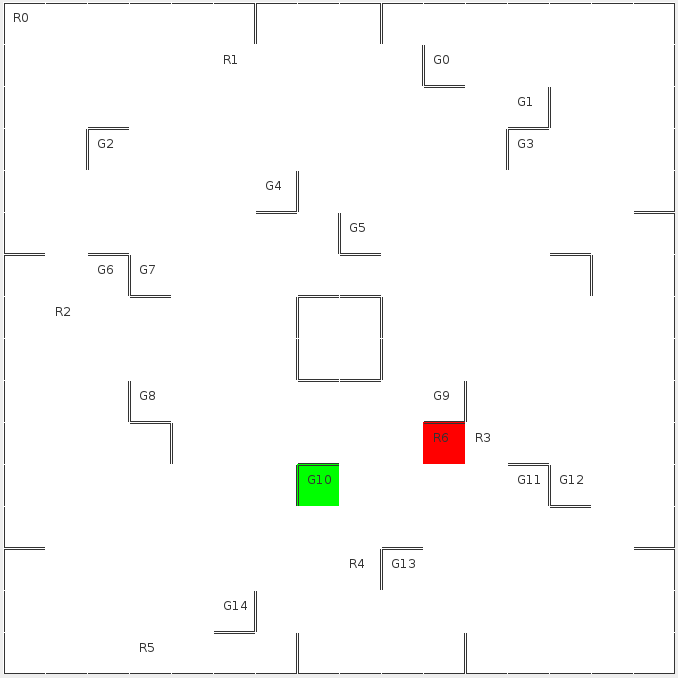
\includegraphics[height=2.6cm, width=10cm]{images/visuBoard.png}}
\institute{Université de Caen Normandie}

\begin{document}

\begin{frame}[plain]
%	\includegraphics[scale= 0.2]{LogoUNICAENv.png}
	\titlepage 
\end{frame}

\begin{frame}[plain]
\Large{Table des matières :}
	\tableofcontents[hideallsubsections]
\end{frame}

%\insertpagenumber %Pour avoir un numéro de page
%%%%%%%%%%%%%%%%%%%%%%%%%%%%%%%%%%%INFOS%%%%%%%%%%%%%%%%%%%%%%%%%%%%%%%%%%%%%%%%%%%%%%%%
%
%Grille d’évaluation de l’oral (5 points) :
%	• Diaporama non surchargé mais présentant des informations pertinentes (1 point)
%	• La présentation orale et la démonstration se sont faites dans les temps (1 point)
%	• Explication claire du projet et des points principaux (1 point)
%	• Démonstration de l’application correctement préparée (1 point)
%	• Réponses correctes aux questions du jury (1 point)
%
%1. Préparez un diaporama  2. Pas de diapositives trop chargées, pas de diapositives %vides    3. Numérotez les diapositives    4. Répartissez-vous équitablement la parole    %5. Ne lisez pas votre texte    6. Tout ce qui est dans le rapport n’a pas vocation à %être à l’oral    7. Mettez en valeur votre réalisation    8. Assurez-vous de la %lisibilité des diagrammes et images    9. Préparez votre démonstration à l’avance %%%%%%(faites une vidéo)
%%%%%%%%%%%%%%%%%%%%%%%%%%%%%%%%%%%INFOS%%%%%%%%%%%%%%%%%%%%%%%%%%%%%%%%%%%%%%%%%%%%%%%%


%MAX 25 diapos !


%--------------Partie 1--------------%
\section{Partie 1 - Introduction, choix du sujet}
	\subsection{Partie 1.1 - Introduction}
\begin{frame}[plain]
\frametitle{Partie 1 : Introduction, choix du sujet}
\framesubtitle{Qu'est-ce que le jeu de Ricochet Robot ?}
C'est un jeu de plateau où un robot doit atteindre une cible en faisant le moins de mouvements possibles.
\begin{figure}
	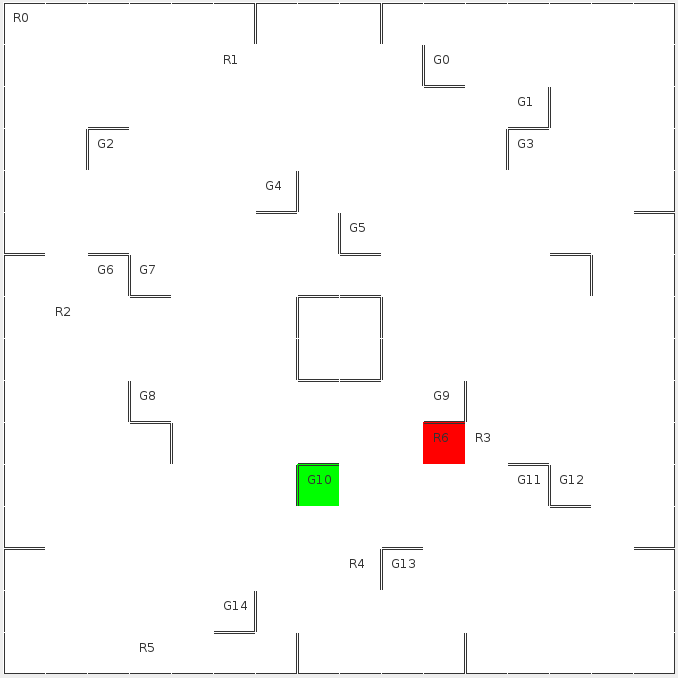
\includegraphics[width=10cm]{images/visuBoard.png}
	\caption{Jeu de Ricochet Robot}
\end{figure}
\end{frame}

	\subsection{Partie 1.2 - Choix du sujet}
\begin{frame}[plain]
\frametitle{Partie 1 - Introduction, choix du sujet}
\framesubtitle{1.2 - Choix du sujet}
\begin{alertblock}{Pourquoi avoir choisi ce sujet ?}
	\begin{itemize}
		\item implémentation d'un algorithme A*
		\item 
	\end{itemize}
\end{alertblock}
\bigbreak
\begin{exampleblock}{Constitution de l'équipe}
Par affinité 
\end{exampleblock}
\end{frame}

%--------------Partie 2--------------%
\section{Partie 2 - Le moteur de jeu}
	\subsection{Partie 2.1 - Le plateau de jeu}
\begin{frame}[plain]
classe Board. Expliquer les cases, 
comment il est construit. addWall
\end{frame}
	\subsection{Partie 2.2 - Les robots et les cibles}
\begin{frame}[plain]
Qu'est-ce qu'un robot ? %et leur mise en place sur le plateau
Qu'est-ce qu'une cible ? %et leur mise en place sur le plateau
\end{frame}
	\subsection{Partie 2.3 - Les déplacements des robots}
\begin{frame}[plain]
Expliquer le déplacement d'un robot
Expliquer la méthode qui le permet
\end{frame}
	\subsection{Partie 2.4 - Autres méthodes nécessaires}
\begin{frame}[plain]
L'aléatoire dans le jeu(au début quand on )
robot présent sur une case? isRobot \& isMainRobot
Est-ce bien l'objectif ? isGoal \& isMainGoal
La fin du jeu. isFinished
\end{frame}

%--------------Partie 3--------------%
\section{Partie 3 : implémentation graphique et structure MVC}
\begin{frame}[plain]
\end{frame}
	\subsection{Partie 3.1 - Notre interface graphique et ce qu'elle contient}
\begin{frame}[plain]
Présentation de l'interface et du JPanel qui contient le Board et la VueMenu.
Explication des boutons
\end{frame}
	\subsection{Partie 3.2 - Fonctionnement de notre structure MVC}
\begin{frame}[plain]
\end{frame}

%--------------Partie 4--------------%
\section{Partie 4 : algorithme A* et BFS}
	\subsection{Partie 4.1 - A*}
		\subsubsection{Partie 4.1.1 - Fonctionnement de A*}
\begin{frame}[plain]
Présentation de l'algorithme A*
\end{frame}
		\subsubsection{Partie 4.1.2 - Implémentation de A*}
\begin{frame}[plain]
Explications sur le A*
\end{frame}
%ajouter autant de frame qu'il faut

	\subsection{Partie 4.2 - Le Breadth First Search ou BFS}
		\subsubsection{Partie 4.2.1 - Fonctionnement du BFS}
\begin{frame}[plain]
Présentation de l'algorithme BFS
\end{frame}
		\subsubsection{Partie 4.2.2 - Implémentation du BFS}
\begin{frame}[plain]
Explications sur le BFS
\end{frame}
%ajouter autant de frame qu'il faut

%--------------Partie 5--------------%
\section{Partie 5 : conclusion}
	\subsection{Expérimentations}
\begin{frame}[plain]
Expérimentations en terme de temps
Expérimentations en terme de coût (nombre de noeuds parcourus)
\end{frame}
	\subsection{Partie 5.1 - Améliorations possibles}
\begin{frame}[plain]
Lister les améliorations possibles
\end{frame}

	\subsection{Pour conclure}
Merci pour votre écoute
logo unicaen
\end{document}
